\section{Modelling Ramping Behaviour Analysis Algorithm} \label{sec:model}

The wind power variations are classified by wind the ramp events. The RBA (Ramping Behaviour Analysis) is an algorithm that determines ramp events based on peak power. This algorithm has four components: rise time, fall time, ramp-up rate and ramp-down rate. The graphical representation in fig. \ref{fig:rba} describes a ramp event and the associated components. The angle ($\theta$) is with reference to the peak point for both up-ramp and down-ramp events. The persistence describes the amount of time the peak event persists. The rise-time and fall-time are presented as $\Delta \; t^{up}$ and $\Delta \; t^{down}$ respectively.

  \begin{figure}[H]
    \centering
    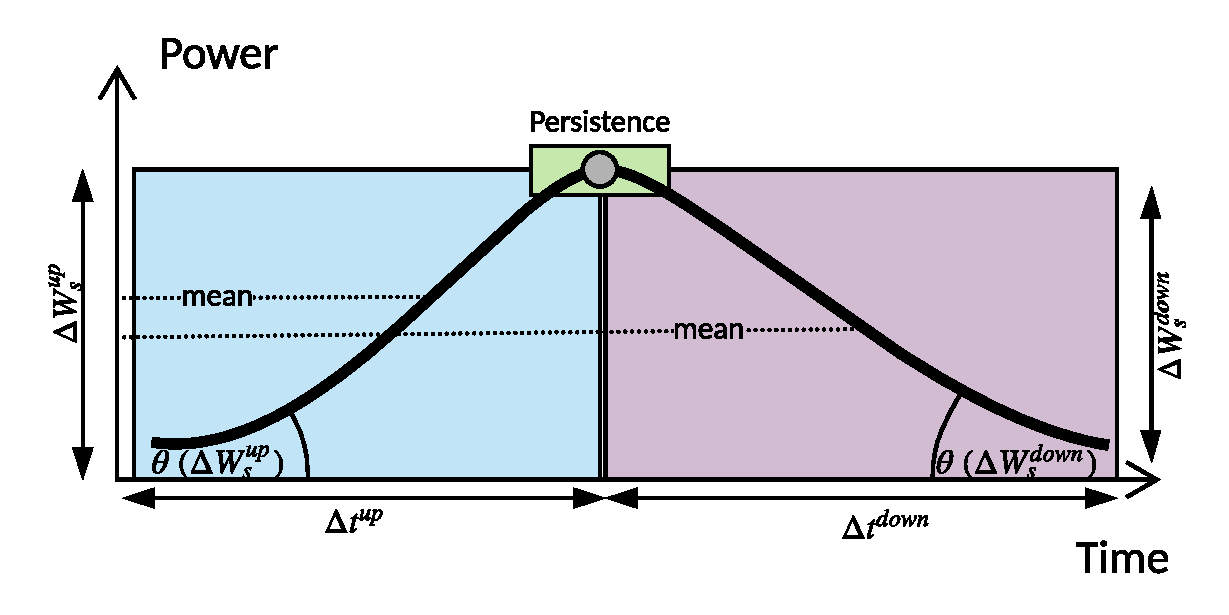
\includegraphics[width=.8\textwidth]{./sec/fig/RBA_new.pdf}
    \caption{Wind ramp event classification}
    \label{fig:rba}
\end{figure}


\subsection{Wind power data}
The data is obtained from the wind park with hourly time resolution. All data points coincide with each other date and time-wise for each turbine. Fig. \ref{fig:wind_data} presents the power output from the wind park for 8760 hours. The data has certainly many power swings and it can be seen more clearly when a smaller time-window is chosen. However, the data is demonstrated with a top-view to show the pattern in seasons. For example, the winter season has dense power power production in comparison to lighter one in summer. 


  \begin{figure}[!htbp]
    \centering
    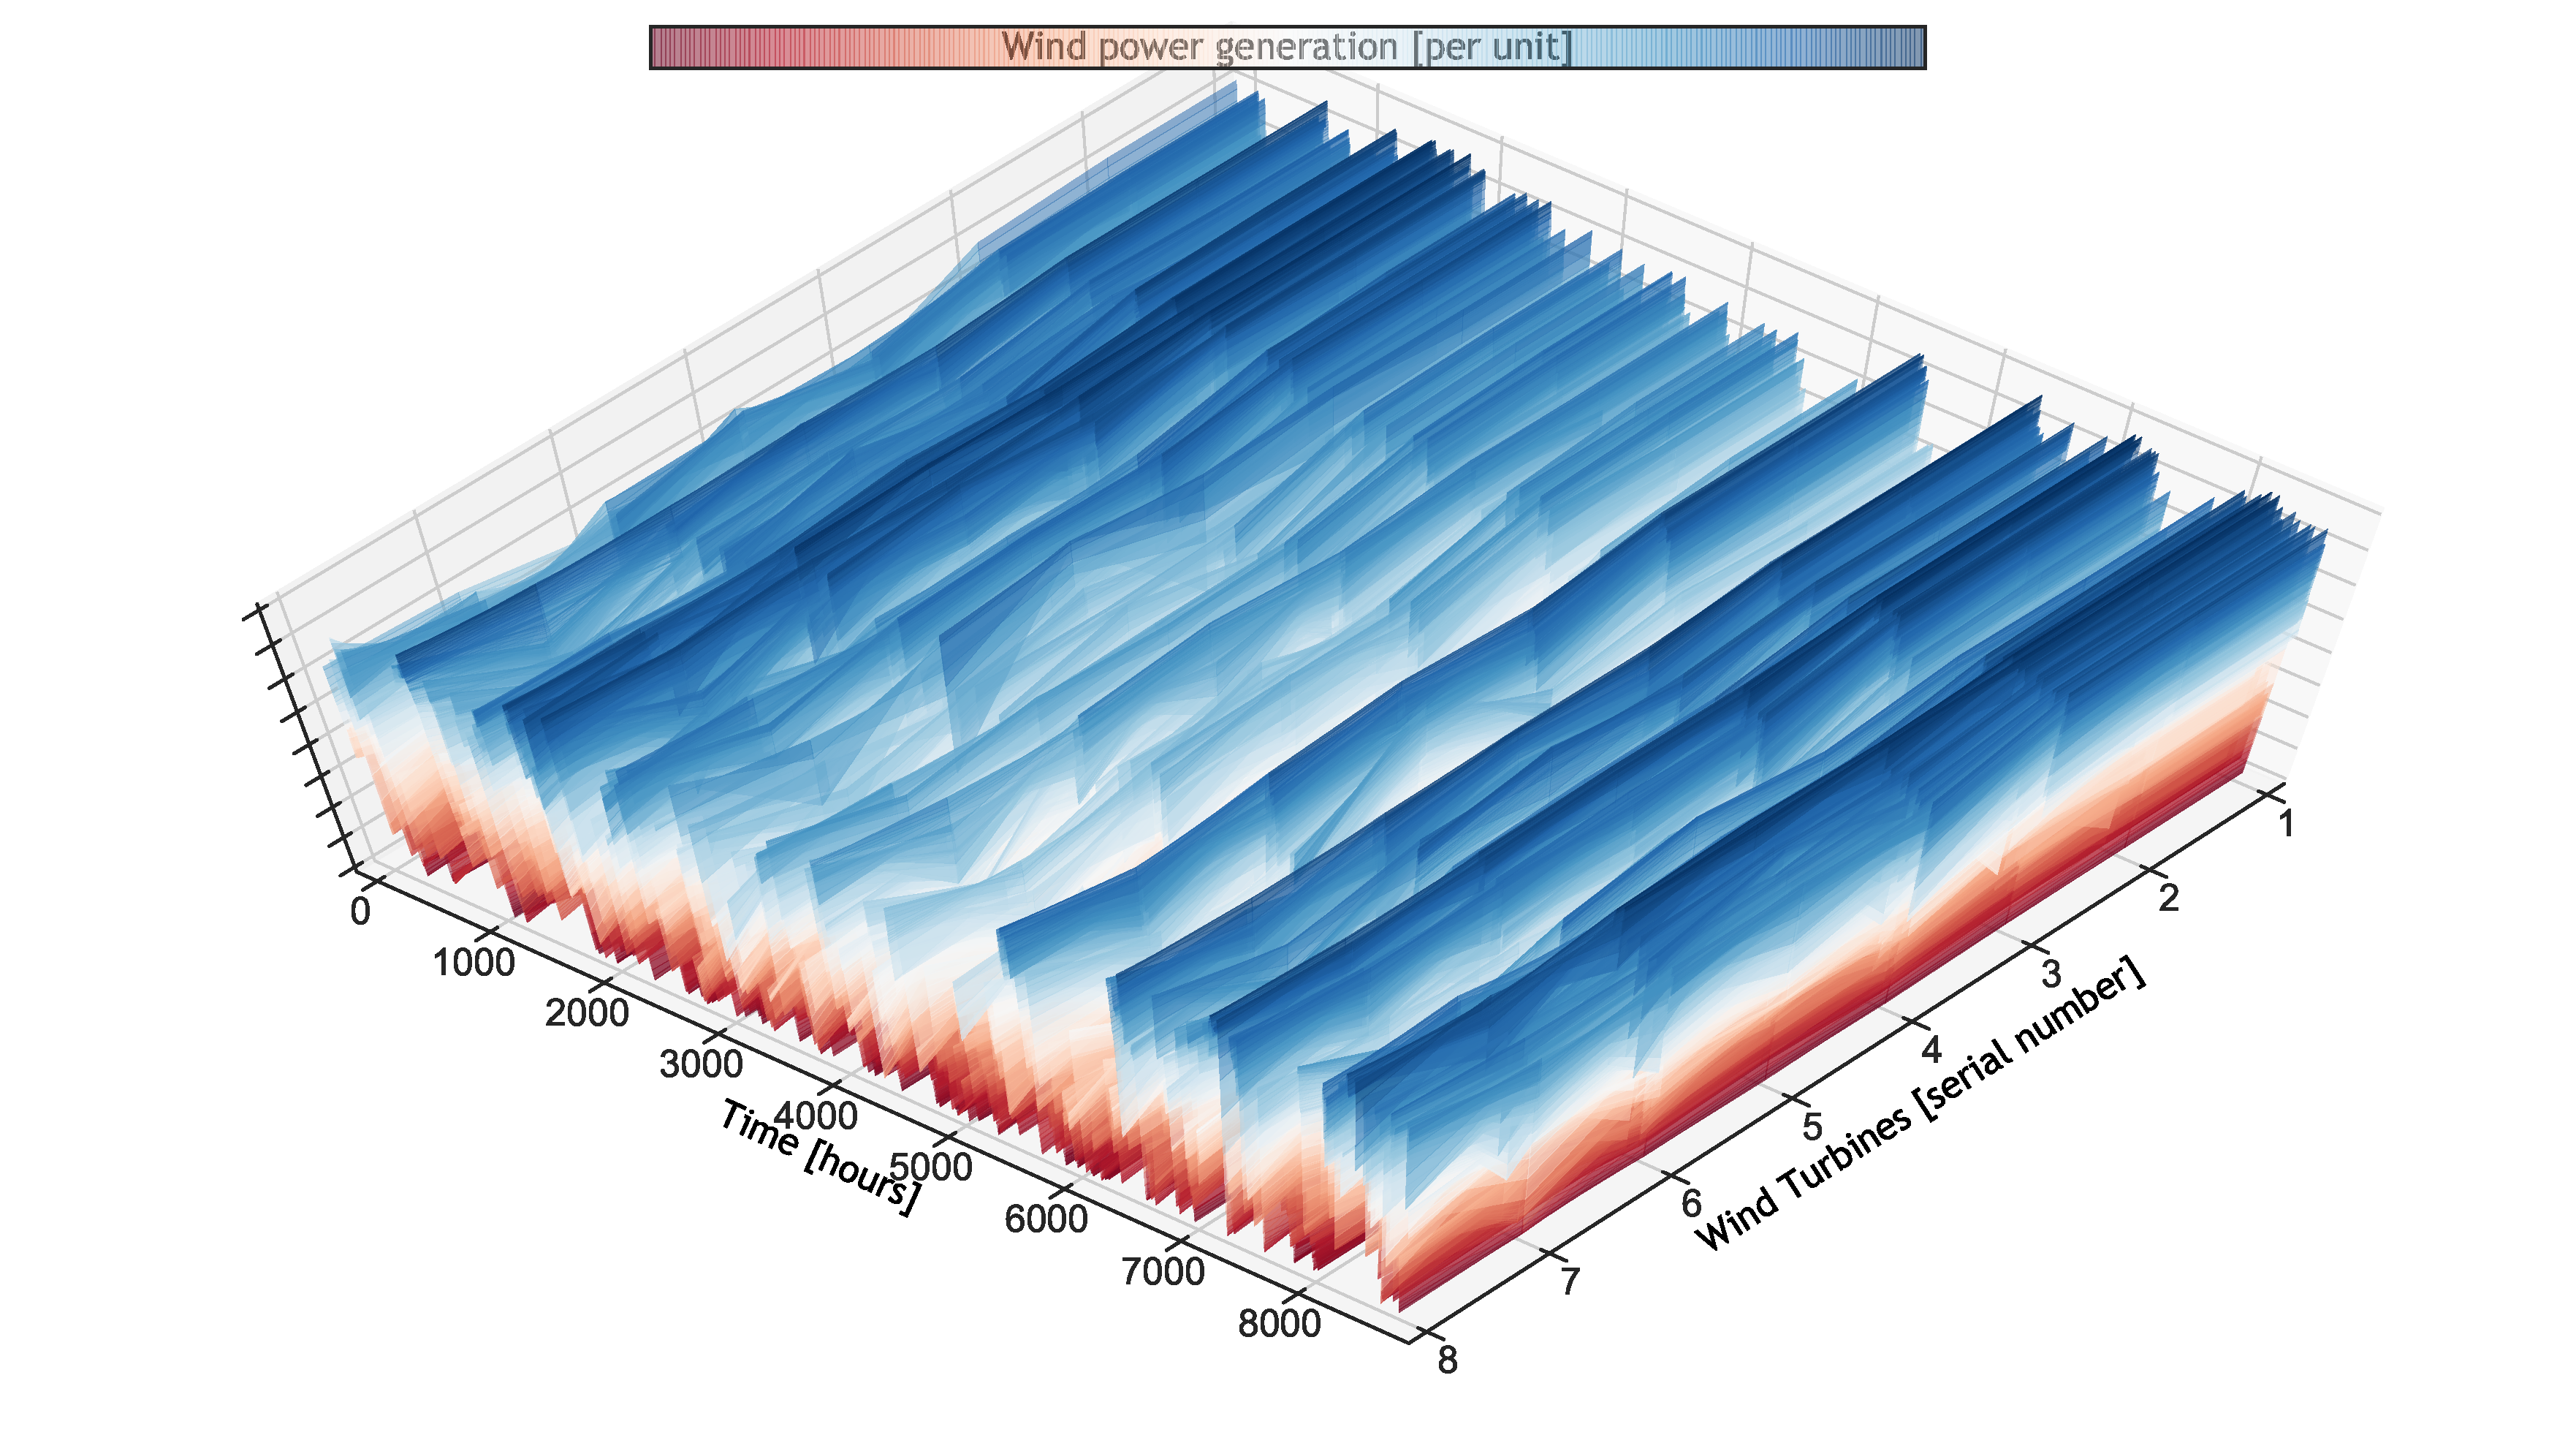
\includegraphics[width=\textwidth]{./sec/fig/wind_data.pdf}
    \caption{Wind power generation from Palidiski wind farm}
    \label{fig:wind_data}
\end{figure}

wind production of a turbine is expressed through capacity factor: the ratio between the net power generation and the calibrated  as in \( \displaystyle \frac{P_{net}}{P_{rated}} \). The data are registered with a time stamp, however the relation between two subsequent observation is not. Again, the degree of noise content that is inherent to the data is substantial for event detection. For example one outlier could either be a significant event. Thus raw data is smoothed through different smoothing techniques to capture the significant events. 

\begin{figure}[!htbp]
 \centering
    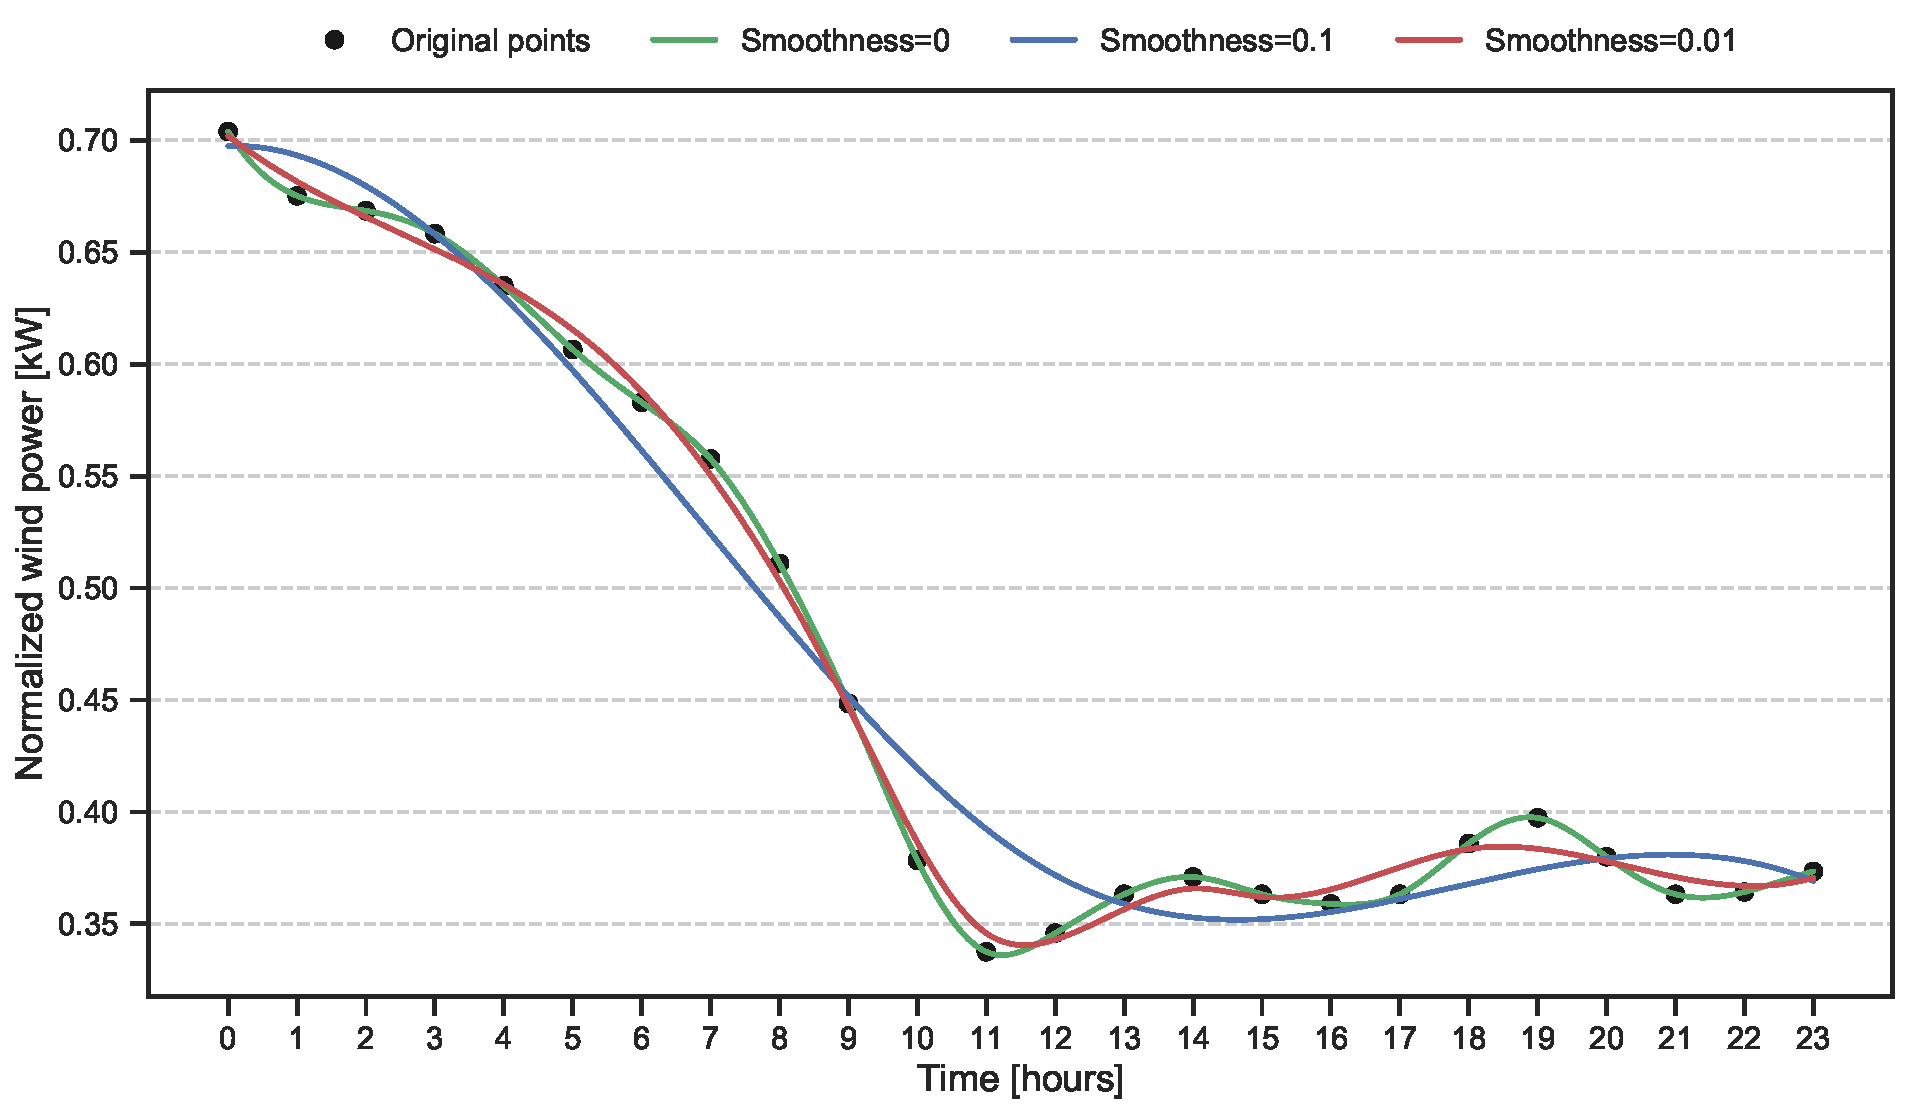
\includegraphics[width=0.8\textwidth]{./sec/fig/Splined_Plot.pdf}
    \caption{Wind power data smoothing using cubic spline smoothing technique}
    \label{fig:data_splined}
\end{figure}

The wind power production data from the wind farm is pre-processed to smoothing technique. A cubic spline method is chosen that is a special case of spline interpolation. In \eqref{eq:spline} presents the $S_i$ cubic spline function. Subsequently the coefficients are obtained starting from $z_0$ and then using the recurrence relation. This technique has smaller error than Newton polynomial and Lagrange polynomial \cite{de1978practical}. In fig. \ref{fig:data_splined} the original data and a comparison between smoothness 0, 0.1 and 0.01 for a 24 hour period is presented. It is evident that smoothness 0.01 is very close to the original trend in the wind power data. 

\begin{subequations} \label{eq:spline}
\begin{align}
S_i (x) & = y_i + z_i (x - x_i) + \frac{z_{i+1} - z_i}{2 * (x_{i+1} - x_i)} (x-x_i)^2  \\
z_{i+1} & = - z_i + 2 * \frac{y_{i+1} - y_i}{x_{i+1} - x_i}
\end{align}
\end{subequations}

%Exponential moving average filter technique is used for smoothing the data as in \eqref{eq:ma}. Here $f, c, p, w$ stands for exponential moving average, current value, previous value and $w=2/(N+1)$ weight factor wherein $N$ is number of periods respectively. The results are presented in the subsequent publication \cite{ArticleNo1}.
%
%\begin{equation}\label{eq:ma}
%    f(c) = \big[ \{ c - f(p) \} w \big] + f(p)
%\end{equation}

A given function or signal can be transformed  from time to frequency domain and other way round. The frequency domain transforms the linear differential to algebraic equations which are easy to solve. Furthermore, the latter provides qualitative behavior of the system: such as bandwidth, frequency response, gain, phase shift, power spectral density, eigenvalues to name a few. The focus on this thesis is limited to spectral density and FFT (Fast Fourier transformation). The Fourier transform of a function contains all the information about the original signal, and with this information, it is possible to reconstruct the function entirely by an inverse Fourier transform. This information includes amplitude and phase of each frequency present in the function. 
The Fourier transform of a discrete-time signal $x[n], n=0,..,N$ is called the discrete-time Fourier transform (DTFT), which provides a mathematical approximation of the full integral solution, and yields a periodic frequency spectrum. The DTFT of the sequence $x[n]$ denoted in  \eqref{eq:filter1} is a function of a continuous frequency variable $\omega$ and $X(e^j\omega )$ and is always periodic with period $2 \pi$. And \eqref{eq:filter2} represents the inverse DTFT of $x[n]$. DFT (Discrete Fourier Transform) can be obtained from the DTFT by evaluating through a discrete set of equally spaced frequencies \cite{mcclellan2003signal}. 

\begin{subequations}
\begin{align} 
\centering
X( e^{j\omega} ) & = \sum_{n=- \infty}^{\infty} x[n] e^{-j \omega n} \label{eq:filter1}\\
x[n]  & = \frac{1}{2 \pi} \int_{- \pi}^{\pi} X( e^{j\omega} ) e^{-j \omega n} d \omega \label{eq:filter2}
\end{align}
\end{subequations}

A finite number of samples are selected to determine the spectrum. Then a window is generated by a multiplication of $x[n]$ by another sequence $w[n]$. Blackman window is selected for the study \cite{agarwal2014mathematical}. A time-domain representation of the same is presented in \eqref{eq:fd} where $N$ is the \textit{length} of Blackman window.

\begin{align} \label{eq:fd}
    w(n) = 0.42 - 5 \cos \left( \frac{2 \pi n}{N-1} \right) +0.88 \cos \left( \frac{4 \pi n}{N - 1} \right) \qquad \forall \; 0 \leq n \leq (M-1) 
\end{align}

\[
 M =
  \begin{cases}
    N/2       & \quad \text{if } N \text{ is even}\\
    (N+1)/2  & \quad \text{if } N \text{ is odd}
  \end{cases}
\]


\begin{figure}[!htbp]
 \centering
    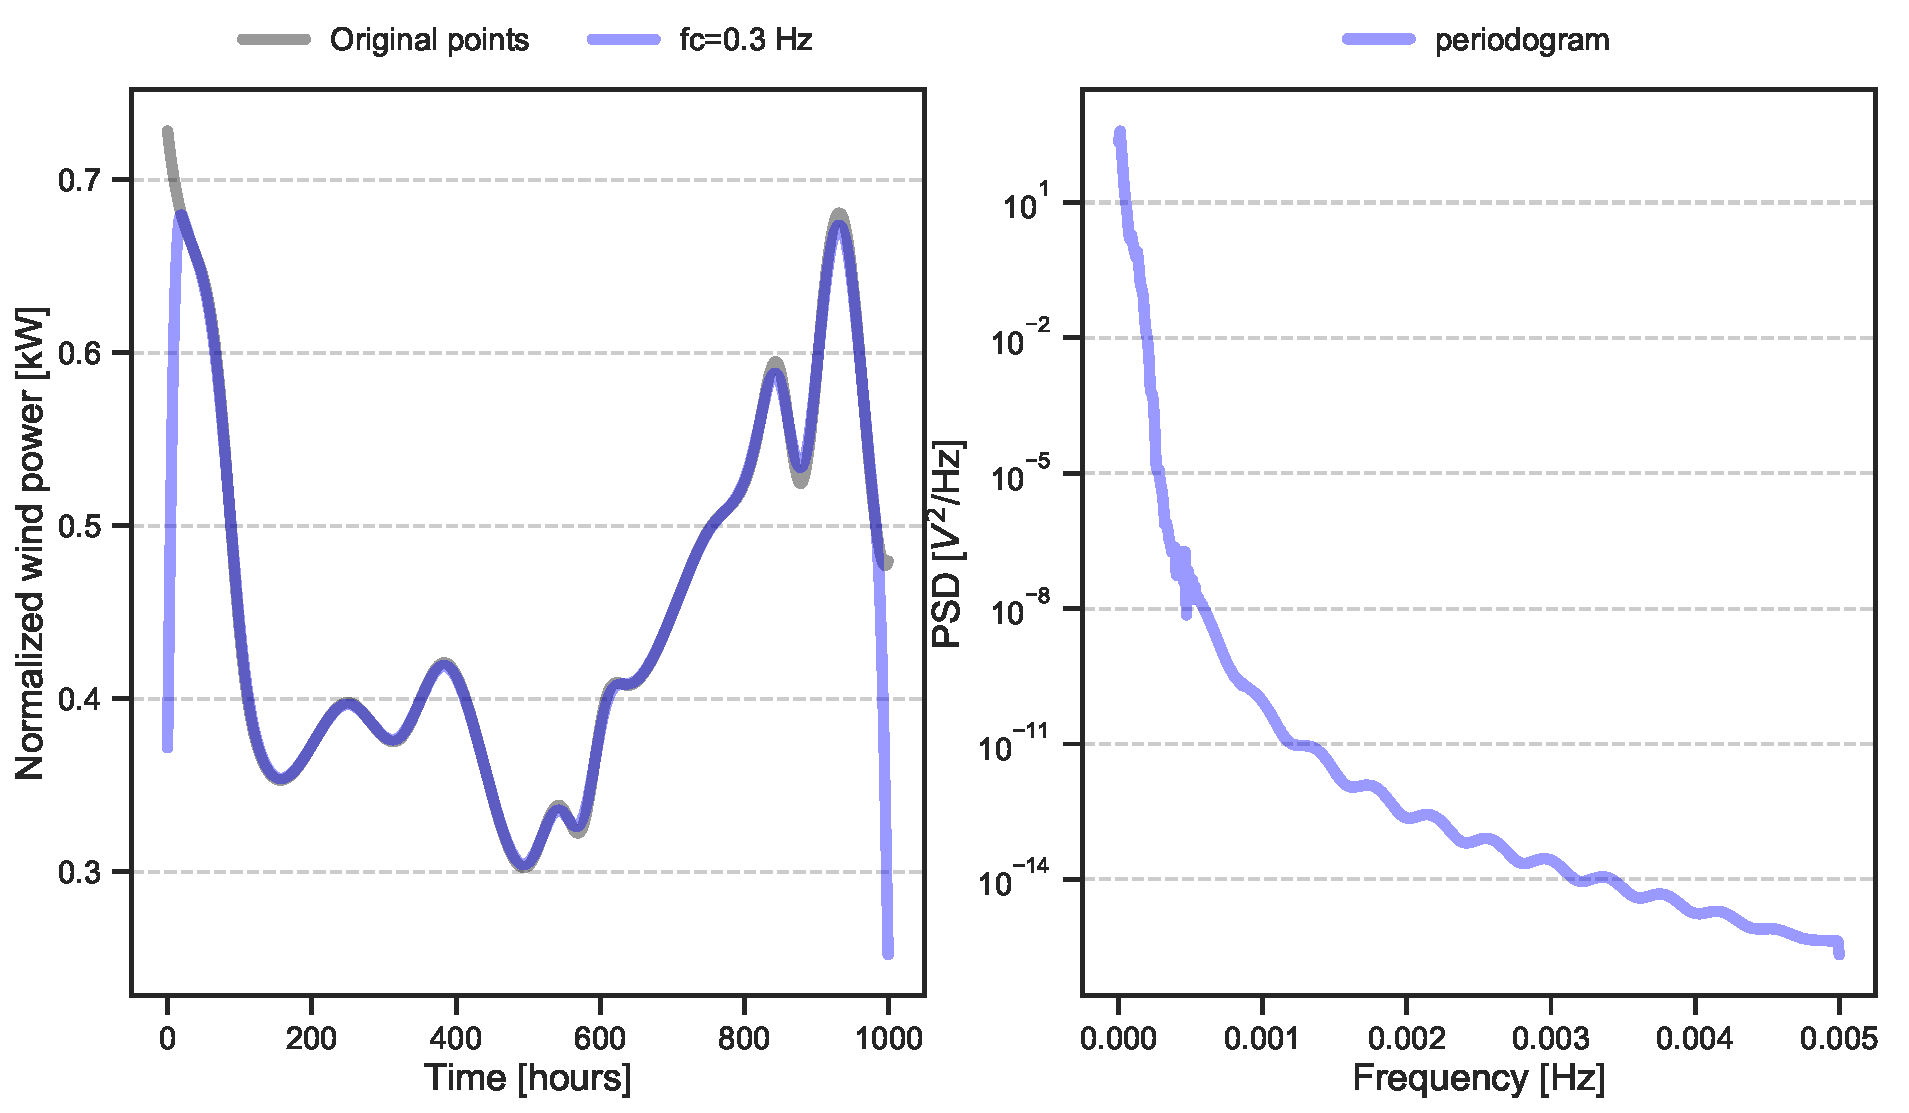
\includegraphics[width=0.8\textwidth]{./sec/fig/Time-to-freq_plot.pdf}
    \caption{Frequency domain transformation: (A) filtered data with 0.3 Hz cut-off frequency (B) periodogram plot showing power spectral density}
    \label{fig:fft}
\end{figure}


%  \begin{figure}[!ht]
%\centering
%\begin{subfigure}{.5\textwidth}
%  \centering
%  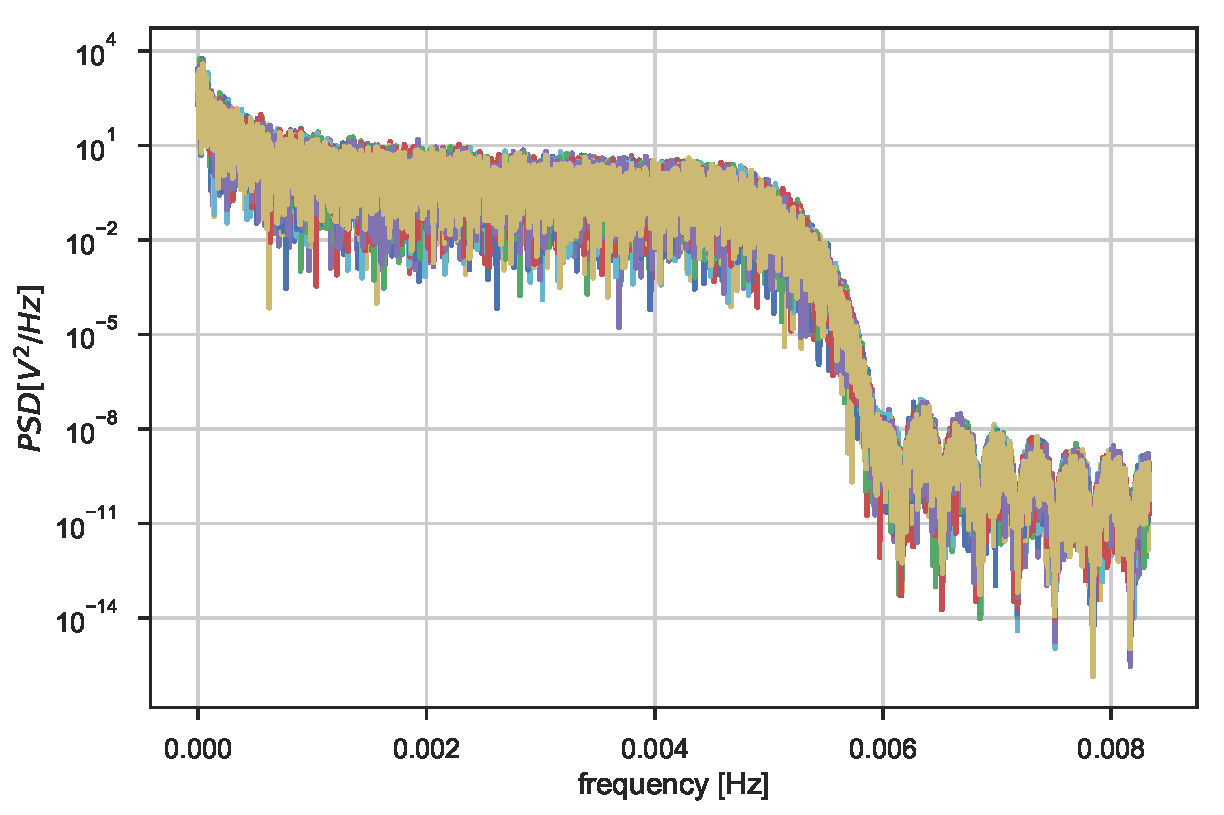
\includegraphics[width=\textwidth]{./sec/fig/periodogram.pdf}
%  \caption{Power spectral density}
%  \label{fig:fft1}
%\end{subfigure}%
%\begin{subfigure}{.5\textwidth}
%  \centering
%  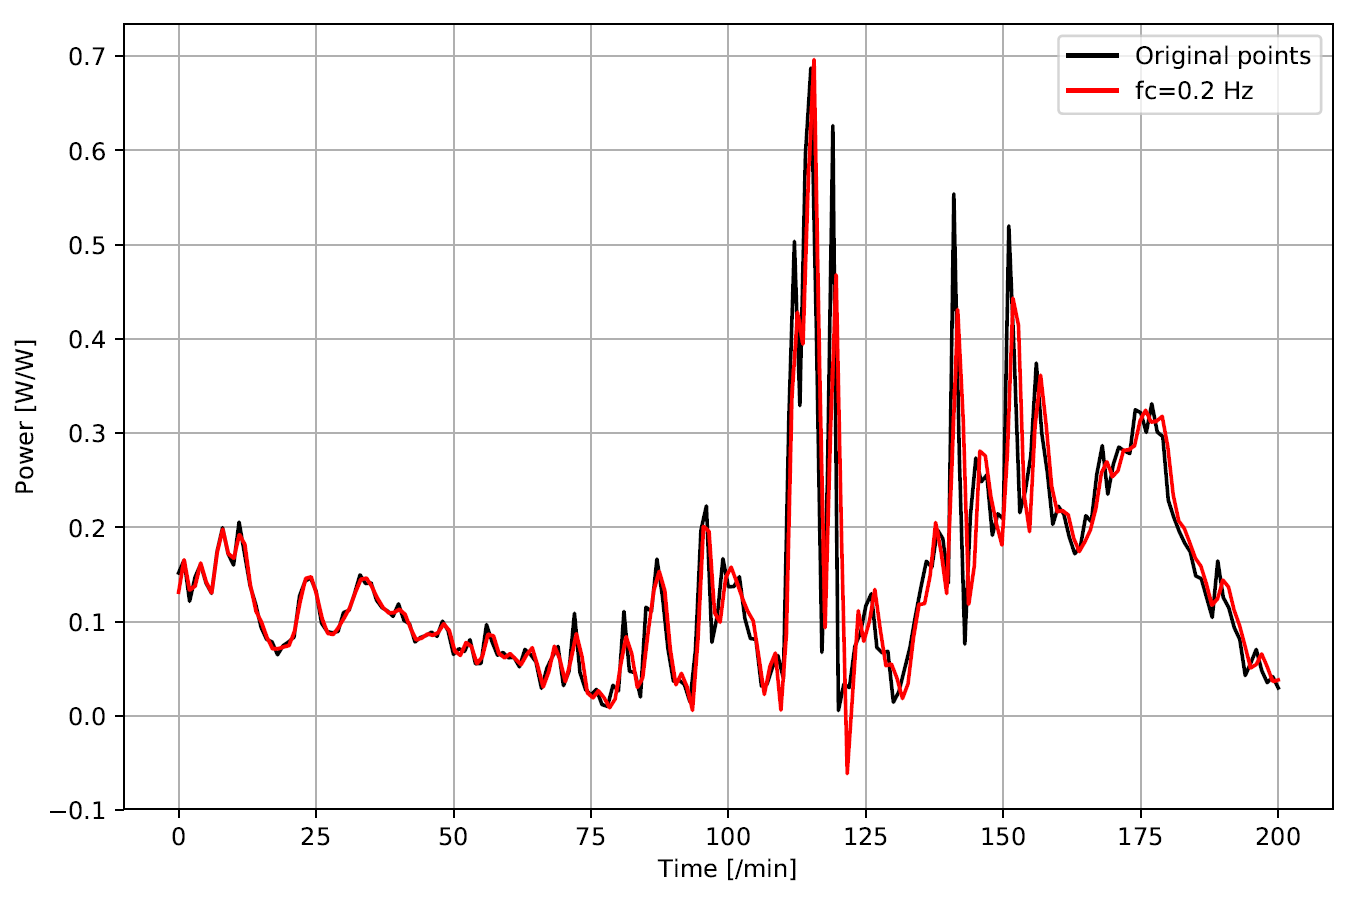
\includegraphics[width=\textwidth]{./sec/fig/fft2.png}
%  \caption{Filtered data with 0.2 Hz cut-off frequency}
%  \label{fig:fft2}
%\end{subfigure}
%\caption{Frequency domain interpretation of cut-off point}
%\label{fig:fft}
%\end{figure}

Fig. \ref{fig:fft} presents the data in frequency domain after the transformation from time to frequency domain. A Blackman window filter is used to remove the noise content in the wind power data. A smaller time window is chosen to demonstrate the changes. In fig. \ref{fig:fft}(A) the original data and data with 0.3 Hz cut-off frequency ($f_s$) is presented. Power spectral density (Welch-periodogram)of $x[n]$ is presented in fig. \ref{fig:fft}(B). 
The data is pre-processed for removing the noise content in the data during measurement. For this, a smoothing technique is used to smooth the data. Following that, a time to frequency domain transformation is performed. In this process, the data is passed through Blackman filter. The subsequent section explains the RBA$_\theta$ and the extraction of events from the original time-series power production.

\subsection{Improved Ramping Behaviour Algorithm}

RBA (Ramping Behvaiour Analysis) is a model to detect wind ramp events. Consider the wind power generation $w_t$ at discrete time $t$ and the consecutive measurement as $w_{t+1}$ where the balance is $w_{\Delta \;t}$. A finite variation $\Delta \; w$ therefore denoted as a ramp. Positive value of $\Delta \; w$ becomes a positive ramp and otherwise is denoted as a negative ramp. 
Thus a ramp event $\Delta \; w_s$ is defined as an event where a significant change in power generation takes place in a time period $\Delta \; t$. The significance is determined through the parameter $T$ that stands for an adjustable threshold to neglect $\Delta \; w$ values that are smaller than a set threshold $T$ as in  $\Delta \; w_s = \Delta \; w \quad | \Delta \; w > T $. A detailed explanation of RBA is presented in the \cite{ArticleNo1},\cite{ArticleNo2}. The mathematical expression for identification of peak points is presented in \eqref{eq:ramp1a}.
 
 
   \begin{figure}[!htbp]
    \centering
    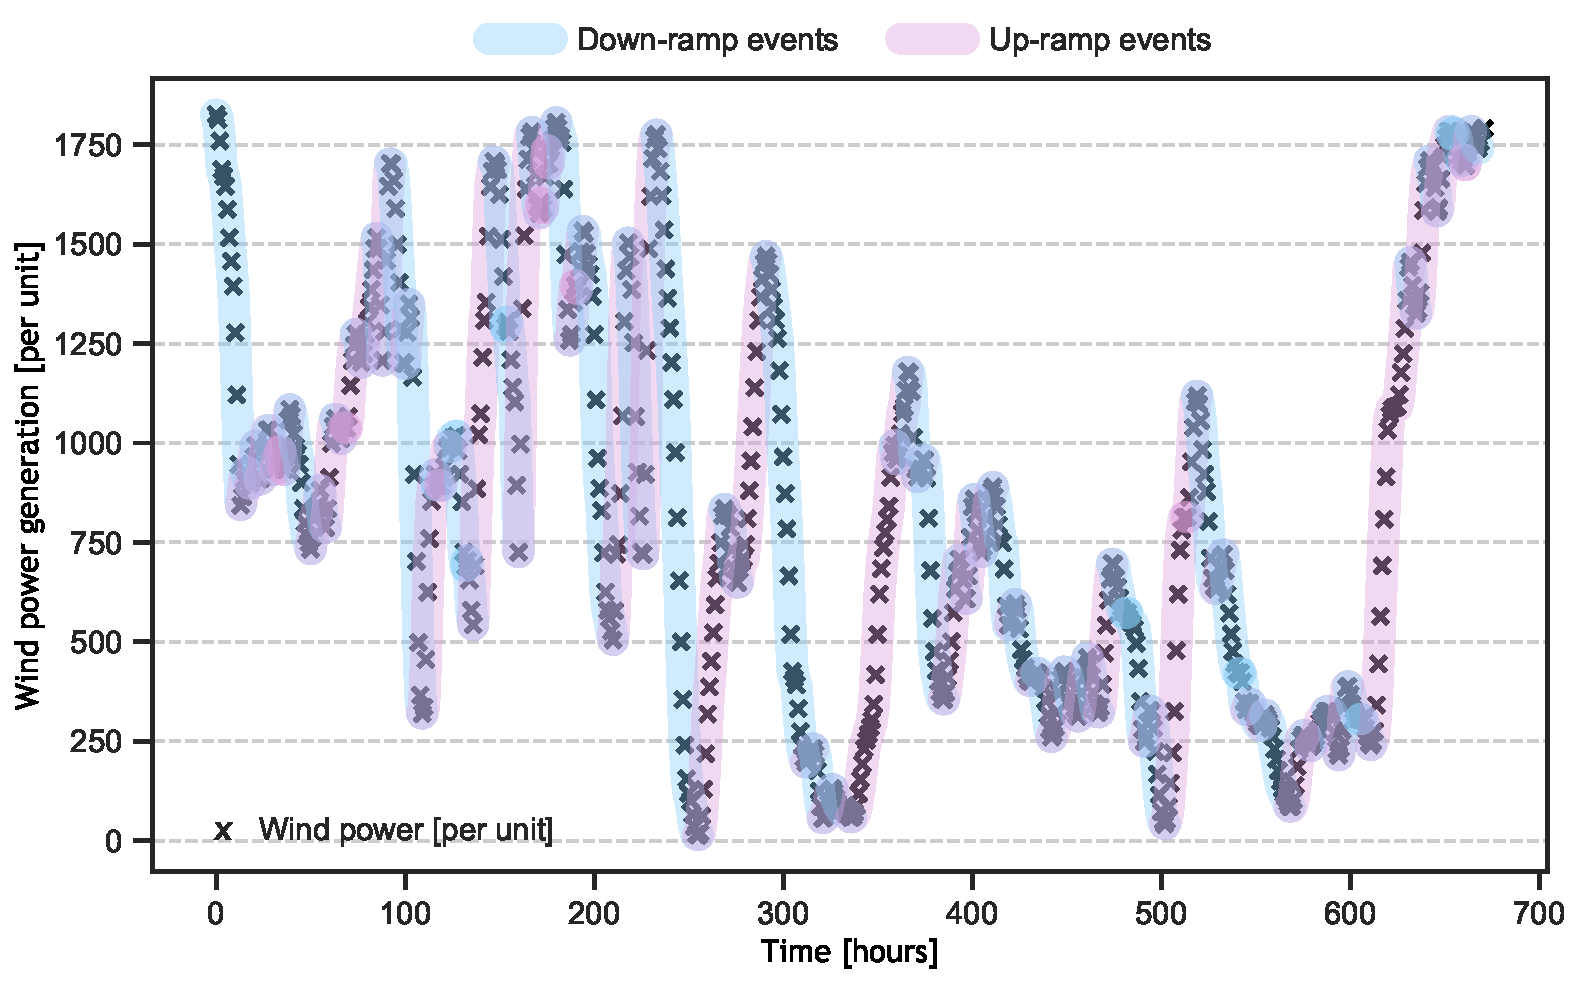
\includegraphics[width=0.9\textwidth]{./sec/fig/RBAevents.pdf}%RBAevents_final.pdf}
    \caption{Wind ramp detection with 5\% threshold}
    \label{fig:ramp_theta}
\end{figure}
% \begin{align} \label{eq:ramp}
%     \Delta \; w_s = \Delta \; w \quad | \Delta \; w > T
% \end{align}
The angle between the interval and the change in amplitude is denoted as $\theta$. It can be formulated as in \eqref{eq:ramp1}. An algorithmic description of the $RBA_\theta$ is presented in algorithm \ref{algo1}. The description includes two functions. The first one extract the events and the second one evaluates the number of occurrences of those events. The algorithm takes the input of time varying wind data (vector), the total length of the time period (scalar). Then the events are identified with respect to peak points and event characteristics: ramp-up, ramp-down, rise-time, fall-time, angle of the peak with respect to adjacent minima and persistence values are the results. The angle $\theta$ between two significant changes $\Delta \; w_s$ and $\Delta \; t$ is presented in \eqref{eq:ramp1b}. 


\begin{subequations} \label{eq:ramp1}
\begin{align}
    \textit{mean} \; ( \Delta w_{s}) & = \bigg( \frac{ w_{s,t} + w_{s, (t + \Delta \; t)}}{2} \bigg) \label{eq:ramp1a}\\
    \theta ( \Delta w_{s}) &= \arctan \; ( \Delta w_{s},  \Delta \; t) \label{eq:ramp1b}
\end{align}
\end{subequations}


%%%%%%%%%%%%%% RBA ALGORITHM
\begin{algorithm}[!htbp] 
\SetKwInOut{Input}{Input}
\SetKwInOut{Output}{Output}
\SetAlgoLined
\KwResult{$w_{s,t}, w_{s, (t+\Delta \; t)}, (t+ \Delta t), \Delta w_s,
 \theta(  \Delta w_s), \text{mean} (\Delta w_s)$, $\Delta w_s^f$,
  $\Delta t_s^f$, $(\theta (\Delta w_s))^f$, $\text{mean} (\Delta w_s^f)$}
\underline{function} $RBA_\theta$ \;
\Input{$ T, w_t \quad \in \mathsf{R}^+ $ }
$\Delta w = w_{ t + \Delta \; t } - w_t$ \;
\For{$i \leftarrow 1$ \textbf{to} \textit{length}( $ \Delta w $ )}{
\If{sign( $\Delta w[i]$ ) == sign( $\Delta w [i+1]$ ) }{
concatenate( $\Delta w$ )}
}
\For{$i \leftarrow 1$ \textbf{to} \textit{length}( $ \Delta w $) }{
\If{ $\Delta w > T$ }{
$\Delta w_s \leftarrow \Delta w$}
}
\For{$i \leftarrow$ \textbf{to} \textit{length}( $\Delta w_s$ ) }{
\If{sign( $\Delta w_s[i]$ ) == sign ( $\Delta w_s [i+1]$ )  }{
concatenate( $\Delta w_s$ )\\
events[i] $\leftarrow w_{s,t}, w_{s, (t + \Delta t)}, t, (t + \Delta t),
\Delta t_s, \theta (\Delta w_s), \text{mean} (\Delta w_s)$}
}
 \caption{$RBA_\theta$ algorithm pseudo code}
 \label{algo1}
\end{algorithm}
%%%%%%%%%%%%%%%%%%%%%%%%%%%%


The threshold $T$ was set to 0.01 or 5\% of the nominal capacity of the wind turbine. Fig. \ref{fig:ramp_theta} presents the resulting ramp event detection. The power production are marked with $x$ marks and ramp-up and ramp-down events are highlighted through blue and purple. Arrows present the scheme used to classify the events, for instance a long red arrow describes a long ramp-up event wherein there are two peak points considered as one significant up event. Note that the first ramp up event persisted for longer period in comparison to the second and third. Similarly the third ramp event persisted for longer period than the other. Clearly persistence values explain the length of an event and thereby indicates the severity. In other words, in a specific period of time if there exists multiple peak points with or without slight difference then the multiple points are counted as one event persisting over that time period.
Note that frequency and persistence are distinct from each other. While the frequency counts the number of occurrences of an event in the time-series data, the persistence values demonstrate how long an event has persisted with respect to time.

\begin{table}[!htbp]
\centering
\begin{tabular}{ccccccccc} \hline
Event & $w_s^t$ & $\Delta \; w_s (t+\Delta t)$ & $t$ & $t+\Delta t$ & $\Delta w_s^t$ & $\Delta t$ & $\theta \Delta w_s$ & $mean(\Delta w_s)$ \\ \hline
01 &	0.580	&	0.798	&	0.000	&	1.000	&	0.218	&	1.000	&	65.340	&	0.689	\\
02 &	0.691	&	0.336	&	14.000	&	123.000	&	-0.355	&	109.000	&	-1.868	&	0.514	\\
03 	&	0.482	&	0.684	&	872.000	&	914.000	&	0.201	&	42.000	&	2.743	&	0.583	\\
04 &	0.684	&	0.126	&	914.000	&	1083.000	&	-0.558	&	169.000	&	-1.891	&	0.405	\\
05 &	0.541	&	0.126	&	1012.000	&	1083.000	&	-0.415	&	71.000	&	-3.347	&	0.333	\\
06 &	0.126	&	0.367	&	1083.000	&	1150.000	&	0.241	&	67.000	&	2.063	&	0.246	\\
07 	&	0.215	&	0.683	&	1348.000	&	1466.000	&	0.468	&	118.000	&	2.270	&	0.449	\\
08 &	0.683	&	0.515	&	1466.000	&	1523.000	&	-0.168	&	57.000	&	-1.685	&	0.599	\\
09 &	0.522	&	0.291	&	1532.000	&	1589.000	&	-0.231	&	57.000	&	-2.320	&	0.407	\\
10	&	0.291	&	0.714	&	1589.000	&	1658.000	&	0.422	&	69.000	&	3.503	&	0.502	\\
\hline
\end{tabular}
\caption{RBA$_\theta$ parameters}
\label{tbl:rba1}
\end{table}

The frequency of occurrence is a measure to count these ramp events in the time horizon of the wind power data. Since this method identifies local peaks in the data with respect to the adjacent minimum point, the first ramp-up event ignores the first peak (at 0.16) and considers the peak at 0.20 in y-axis. Consequently the adjacent minimum point 0.13 is ignored and 0.12 is recorded. There is an overlap of the events at the meeting point this is because the event length includes both the starting and end point of the wind power data. In this way, events are aligned end-to-end. With that, $RBA_\theta$ identifies and counts the events while recording the event details at all stages. The table \ref{tbl:rba1} presents the RBA$_\theta$ parameters for 10 sample events.  